
\documentclass{article}
\usepackage[utf8]{inputenc}
\usepackage{biblatex}
\addbibresource{referencias.bib}

\usepackage{hyperref}
\usepackage[spanish, es-tabla]{babel}

\usepackage{authblk}
\renewcommand\Authand{ y }
\renewcommand\Authands{, y }
\renewcommand*{\Authfont}{\bfseries}
%% Page settings
\usepackage[a4paper, margin=1in]{geometry}
\usepackage{graphicx}
\usepackage{float}
\usepackage{caption}
\usepackage{subcaption}
\usepackage{lipsum}
\usepackage{wrapfig}
\usepackage{booktabs}
\usepackage{siunitx}
\DeclareSIUnit{\calorie}{cal}
\usepackage{amsmath}
\usepackage{multicol}
\renewcommand{\d}{\text d}
\newcommand{\dd}[2]{\frac{\d #1}{\d #2}}


\newcommand{\myfigure}[4][0.65]{%
    \vspace{1em}
    \noindent\begin{minipage}{\linewidth}%
        \makebox[\linewidth]{%   For centring figures
            \includegraphics[width=#1\linewidth]{#2}}
        \captionof{figure}{#3}
        \label{#4}
    \end{minipage} 
    \vspace{0.5em}}

\usepackage{amsfonts}
\newcommand{\overbar}[1]{\mkern 1.5mu\overline{\mkern-1.5mu#1\mkern-1.5mu}\mkern 1.5mu}

\usepackage{amsmath}
\everymath{\displaystyle}

\title{\vspace{-15mm}\fontsize{24pt}{10pt}\selectfont\textbf{Equivalentes del Calor}} % Article title 

\author{Andres David Rojas Lozano}
\author{Andres Esteban Leal Buitrago}
\author{Gabriel Sandoval Velasquez}
 
\affil{Universidad Nacional de Colombia}
\affil{\{
    \href{mailto:androjaslo@unal.edu.co}{androjaslo}, 
    \href{mailto:aelealb@unal.edu.co}{aelealb}, 
    \href{mailto:gfsandovalv@unal.edu.co}{gfsandovalv}
    \}@unal.edu.co}

\date{\today}

\setlength{\parindent}{0pt}
\begin{document}
\maketitle
%\begin{multicols}{2}
\begin{abstract}
 
\end{abstract}
\section{Introducción}
\subsection{Capacidad calorífica}
La capacidad calorífica de un sistema puede ser determinada cuando un sistema que absorbe calor tiene una variación de temperatura inicial $T_i$ a una temperatura final $T_f$, es durante dicha transferencia de calor $\delta Q$ que se determina:
\begin{align}
    C=\frac{\delta Q}{T_f-T_i}
\end{align}
Que teniendo valores cada vez más pequeños para dichas variaciones, tendremos:
\begin{align}
    C=\frac{\delta Q}{\Delta T}
\end{align}
Se nota de tal forma que  la capacidad calorífica,se puede definir como el cociente entre la cantidad de energía calorífica transmitida sobre el cambio de temperatura. Es decir, la cantidad de energía necesaria para cambiar la temperatura en una unidad de un determinado sistema.\cite{juleve}
En general, la capacidad calorífica depende de la temperatura como de la presión. Si se sigue un proceso cuasi-estático, se tendrá:
\begin{equation}
    \Delta Q= dU+\Delta W=du+PdV
\end{equation}


\subsubsection{Calor específico (capacidad calorífica específica)}
La versión intensiva de la ecuación \eqref{eq:capacidad_calo} introduciendo el cambio de variable $C=mc$ siendo $m$ la masa del cuerpo y $c$ su calor específico, el cual, evidentemente, es independiente de la masa. Haciendo este cambio, se tiene

\begin{equation}
    \begin{aligned}
        c &= \dfrac{1}{m}\dfrac{\delta Q}{\Delta T} \\
        \delta Q &= m c \Delta T
    \end{aligned}
\end{equation}

En general, por la primera ley, $\delta Q = \d{U} + \delta W$, este diferencial de calor toma formas distintas para dos casos: presión constante y volumen constante. Cuando el volumen es constante, $\delta W = P\d V = 0$, mientras que si la presión es constante $\delta Q = \d H = \d{(U + PV)}$. De aquí que

\begin{align*}
    c_v &= \frac{1}{m}\left(\ddp{U}{T}\right)_v \\
    c_p &= \frac{1}{m}\left(\ddp{H}{T}\right)_p
\end{align*}

Para un proceso cuasi-estático arbitrario entre los estados $A$ y $B$,

\begin{equation}
    c_c = \lim_{A\to B} \frac{1}{m}\left(\frac{Q}{\Delta T}\right)_c =  \frac{1}{m}\left(\frac{\delta Q}{\d T}\right)_c
\end{equation}

\subsection{Proceso adiabático en el calorímetro}

El calorímetro es básicamente un recipiente aislado térmicamente de modo que se considera que tiene paredes adiabáticas. Teniendo en cuenta esto, se puede asegurar (idealmente) que no se intercambia energía con el exterior y que el calor intercambiado se da solamente entre el calorímetro y la muestra,

\begin{align*}
    \delta Q_{\text{calorímetro}} + \delta Q_{\text{muestra}} = 0 \\
    \left(M+ k \right)(T_f-T_0)c_{\text{agua}} + (mc)_{\text{muestra}}(T_f-T) = 0
\end{align*}
Donde $k=(mc)_{\text{cal.}}/c_{\text{agua}}$ es el equivalente en agua del calorímetro, $T_0$ es la temperatura inicial del agua en el calorímetro, $T$ es la temperatura inicial de la muestra y $T_f$ es la temperatura de equilibrio que se alcanza luego de un tiempo. Entonces, para la muestra se obtiene que $c_{\text{muestra}}$

\begin{equation}
c_{\text{muestra}} = c_{\text{agua}}\dfrac{M + k}{m_{\text{muestra}}}\dfrac{T_f-T_0}{T-T_f}
\end{equation}
\subsection{Temperatura de Debye}

Ene los sólidos cristalinos a temperatura ambiente se tiene una capacidad calorífica que es constante, apróximadamente 3R, donde $R=N_ak_B$ con $N_a$ el número de avogadro y $k_B$ la constante de Boltzmann, esto es conocido como la ley de Dulong-Petit, que encaja en las predicciones del teorema de equipartición de la energía.

Einstein fue la primera persona en proporcionar una deducción de la capacidad calorífica de los sólidos. Tiempo después, Debye propuso una mejora para la teoría de Einstein, prediciendo la capacidad calorífica molar de forma:

\begin{equation}
    \frac{C_v}{R}(\frac{\Theta_E}{T})^2(\frac{e(\frac{\Theta_E}{T})}{(\Theta_E-1)^2})^4
\end{equation}
Con $\Theta_E$ es un parámetro conocido como la característica de Einstein del sólido. En general el modelo de Einstein funcionaba bien en un amplio intérvalo de temperatura, sin embargo en 1912 cuando Debye aborda el problema teniendo en consideracipon la propagación de vibraciones moleculares en el material, se tiene :
\begin{align}
    C_v=\frac{9N_ak_B}{\Theta_D^3}\frac{\partial}{\partial T}(T^4 \int_{0}^{\frac{\Theta_D}{T}} \frac{x^3}{e^x-1}dx)
\end{align}
con $k_B\Theta_D$:
\begin{equation}
    k_B\Theta_D=h(\frac{2}{c^3_t}+\frac{1}{c^3_t})^\frac{-1}{3}
\end{equation}
Dónde $\Theta_D$ corresponde al modo normal de oscilación más alto, es decir, la temperatura más alta que puede ser alcanzada con un solo modo normal de vibración para el sistema.

\section{Descripción experimental y procedimiento}

Las mediciones de esta práctica fueron realizadas en dos sesiones,midiendo los calores específicos de diversas muestras de diferentes materiales: Hierro, aluminio y cobre.

Teniendo de este modo:
\subsection{Estimación capacidad calorífica a temperatura ambiente}
Se dispone entonces de un modulo de termocupla el cual trabaja en un rango de 200mV cuya medida retorna valores en grados Celsius, un vaso calorímetro cuya masa es de 48.8g teniendo una disposición experimental como se ilustra en la figura \ref{fig:disp}

Para medir el calor específico de las muestras a temperatura ambiente (apróximadamente 19°), se realiza :
\begin{enumerate}
    \item Se dispone de una cantidad de agua en un recipiente, suficiente para cubrir la muestra, y se calienta por medio de una estufa hasta que este alcance el punto de ebullición del agua, en dicho punto, se mide la temperatura y se extrae la muestra.
    
   \item En el vaso calorímetro se vierte una masa de agua que apenas cubra la muestra, se mide su temperatura.
     
    \item Finalmente es introducida la muestra en el vaso calorímetro, midiendo la temperatura de equilibrio.
     
\end{enumerate}


\begin{table}[]
    \centering
    \begin{tabular}{|c|c|}
    \hline
         Material&Masa(g)$\pm$ 0.1  \\\hline
         Hierro&51.6\\
         Aluminio&17.4\\
         Cobre&19.8\\
\hline
    \end{tabular}
    \caption{Masas de las muestras usadas en la práctica}
    \label{tab:masas}
\end{table}
La conservación de la energía implica que el calor absorbido por el agua y el calorímetro debe ser igual al calor cedido por la muestra.
    
    Se define de esta manera:
    
    \begin{align*}
        m_c&:= \textrm{masa calorímetro}\\
        m_a&:= \textrm{masa de agua en calorímetro}\\
        m_m&:= \textrm{masa muestra}\\
    \end{align*}
Así tendremos en la ecuación \ref{eq:masas} 

\begin{equation}
    m_mc_m(T_{eq}-T_i^{(m)})=(c_{cal}m_{cal}+c_{ag}m_{ag})(T_{eq}-T_i^{(c)})
\end{equation}

Despejando para $c_m$:
\begin{equation}
    c_m=\frac{m_{cal}c_{cal}+m_{ag}c_{ag}}{m_m}\frac{(T_{eq}-T_i^{(c)})}{T_{eq}-T_i^{(m)}}
\end{equation}

\subsection{Calor específico a bajas temperaturas}
Para la medición del calor específico a bajas temperaturas, se hace uso de 2 vasos de poliestireno expandido, conocido localmente como Icopor, el cual tiene por contenido nitrógeno el cual se encuentra en constante estado de evaporación.

Se establece inicialmente una medición para determinar la tasa de evaporación del nitrógeno, el cual se puede establecer es apróximadamente constante, esto relizando una constante medición de la masa perdida por evaporación.
Posteriormente son introducidas una a una las muestras , lo cual aumenta dicha taas de evaporació , que en unos primeros instantes se muestra con una reacción bastante (fuerteJOJOJO)  esto debido a que se produce un intercambio de energía térmica entre la muestra y el nitrógeno, posteriormente, la tasa de evaporación vuelve a ser constante una vez la muestra alcanza la temperatura de ebullición del nitrogeno.

Dado que la temperatura ambiente a la que es introducida la muestra es considerablemente mayor al punto de ebullición del nitrógeno, se presenta en la interacción el efecto Leidenfrost.

La masa evaporada por el intercambio de calor con la muestra, se calcula como :
\begin{equation}
    \Delta m L_{ev}=C_p(T_i-T_f)
\end{equation}
Con $C_p$ la capacidad calorífica  a presión constante, $T_i$ la temperatura de la muestra antes de ser sumergida en el nitrógeno.  El calor latente de evaporación del nitrógeno es $L_{ev}=99.7 J \cdot g^{-1}$.

\subsection{Temperatura de Debye}
\section{Resultados y análisis}
\subsection{Calor específico a temperatura ambiente}
Tras realizas las mediciones para cada muestra, haciendo uso de la ecuación \ref{eq:masas} se determina el calor específico para cada material consignado en la tabla \ref{tab:cp}:

\begin{table}[H]
    \centering
    \begin{tabular}{|c|c|c|c|c|}
    \hline
        Muestra&T_0 Agua &T_{masa} &T_{eq} &c_{p} (J/g K) \\\hline
        \multirow{4}{*}{Hierro}&21.5 &91.0 &28.1  &0.101 \\
        &21.5 &93.8 &26.8&0.108  \\
        & 22.2& 94.2&  27.4&0.097 \\
        & 22.2& 94.0&  27.0&0.096 \\\hline
        \multicolumn{4}{|c|}{Valor promedio}&0.101\\\hline
        \multirow{4}{*}{Cobre}&22.6 &94.4 &28.0 &0.264  \\
        &22.6 &95.0 &28.0 &0.248 \\
        & 22.9& 94.0&27.7 & 0.216\\
        &22.9 & 94.4& 25.5&0.126 \\
        \hline
        \multicolumn{4}{|c|}{Valor promedio}&0.195\\\hline
        \multirow{4}{*}{Aluminio}&22.1 & 94&26.6 &0.192  \\
        & 21.9&94 &26.1 &0.193  \\
        & 22.0&94 &25.7 & 0.187 \\
        & 21.3& 94& 25.2& 0.207 \\
        \hline
     \multicolumn{4}{|c|}{Valor promedio}&0.214\\\hline
     
    \end{tabular}
    \caption{Medicion temperaturas y cálculo de c_{p}}
    \label{tab:cp}
\end{table}

De este modo,

\subsection{Capacidad calorífica a bajas temperaturas}

\begin{figure}
    \centering
    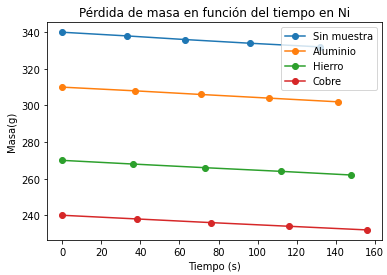
\includegraphics[scale=0.8]{img/nitro.png}
    \caption{Caption}
    \label{fig:my_label}
\end{figure}
\begin{figure}
    \centering
    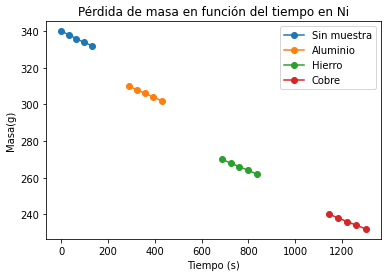
\includegraphics[scale=0.8]{img/nitro2.png}
    \caption{Caption}
    \label{fig:my_label}
\end{figure}
\section{Conclusiones}
\begin{itemize}
    \item El montaje experimental usado para el equivalente eléctrico es bastante sensible al cambio de voltaje. Usando el criterio de la mayor incertidumbre, se obtiene $J_{\text{elec}} = 1.323 \pm 0.014$
\end{itemize}
%\end{multicols}
\printbibliography
\end{document}